
\subsection{Winkel im rechtwinkligen Dreieck: $\sin()$, $\cos()$ und
  $\tan()$}\index{Sinus}\index{Cosinus}\index{Kosinus}\index{Tangens}


\subsection*{Lernziele}
\begin{itemize}
 \item Ähnliche rechtwinklige Dreiecke haben die selben Winkel
 \item Sinus, Cosinus, Tangens
\end{itemize}
Voraussetzungen: 
\TadBMTG{89}{6.2}

\TadBMTG{90}{6.3}
\newpage

\subsection{Ähnlichkeit im rechtwinkligen Dreieck}
Schätzen Sie in den folgenden Dreiecken den Winkel $\beta$:

\bbwCenterGraphic{6cm}{tals/trig1/img/Ae10.png}
$$\beta\approx \LoesungsRaum{30\degre - 31\degre}$$

\bbwCenterGraphic{3.5cm}{tals/trig1/img/Ae11.png}
$$\beta\approx \LoesungsRaum{59\degre - 60\degre}$$

\bbwCenterGraphic{6cm}{tals/trig1/img/Ae12.png}
$$\beta\approx \LoesungsRaum{30\degre - 31\degre}$$

\bbwCenterGraphic{4cm}{tals/trig1/img/Ae13.png}
$$\beta\approx \LoesungsRaum{45\degre - 46\degre}$$

\newpage
\subsubsection{Ähnliche Dreiecke}
\begin{gesetz}{Ähnliche Dreiecke}{}
In ähnlichen Dreiecken sind die entsprechenden Winkel
identisch. Zusätzlich gilt:

$$\frac{b}{a} = \frac{b'}{a'} = \text{ konstant}$$
\end{gesetz}

\begin{tabular}{ccc}
  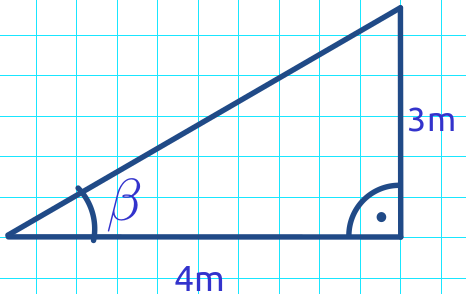
\includegraphics[width=4cm]{tals/trig1/img/Ae20.png} & 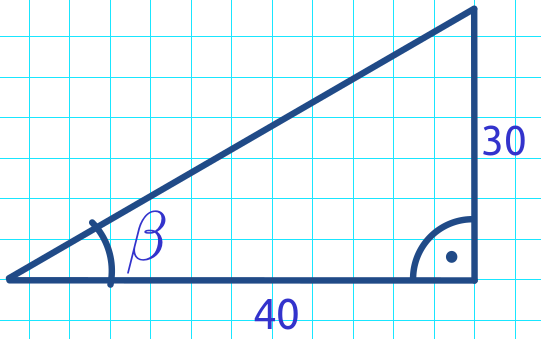
\includegraphics[width=4cm]{tals/trig1/img/Ae21.png} & $\beta\approx$ \TRAINER{$36.87\degre$} \noTRAINER{..........}
\end{tabular} 

\begin{gesetz}{Seiten und Winkel im rechtwinkligen Dreieck}{}
Im rechtwinkligen Dreieck reicht es, zwei Seiten zu kennen, um die
Winkel zu bestimmen.
\end{gesetz}


\subsubsection{Seitenverhältnis}\index{Seitenverhältnis!im rechtwinkligen Dreiech}
Es gilt auch die Umkehrung:
\begin{gesetz}{Seitenverhältnis}{}
Ist in einem rechtwinkligen Dreieck $\alpha$ oder $\beta$ bekannt, so
sind die \textbf{Seitenverhältnisse} eindeutig bestimmt.
\end{gesetz}

\newpage
\subsubsection{Tangens}\index{Tangens}

\begin{definition}{Tangens}{}
Das zu einem Winkel gehörige \textbf{Seitenverhältnis} der beiden
Katheten (gegenüberliegende Kathete zu anliegender Kathete) wird als

\begin{center}\textbf{Tangens} des Winkels\end{center}
  bezeichnet.
\end{definition}
Es gilt:

\begin{gesetz}{Tangens}{}
  $$tan(\beta) = \frac{\text{Gegenkathete} b}{\text{Ankathete} a}$$
\end{gesetz}

Beispiele (berechnen Sie mit dem Taschenrechner):

\begin{tabular}{ccccc}\hline
  Beispiel & Winkel & Verhältnis $\frac{b}{a}$ & $\tan()$ \& Schätzung \\\hline 
 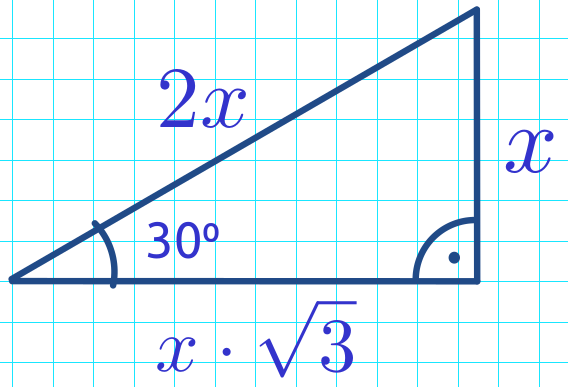
\includegraphics[width=4.5cm]{tals/trig1/img/tan01.png} & $30\degre$ &  \TRAINER{$1 : \sqrt{3}$}\noTRAINER{..........} & $\tan(30\degre) \approx$ \TRAINER{$0.5774$}\noTRAINER{..........}\\\hline
 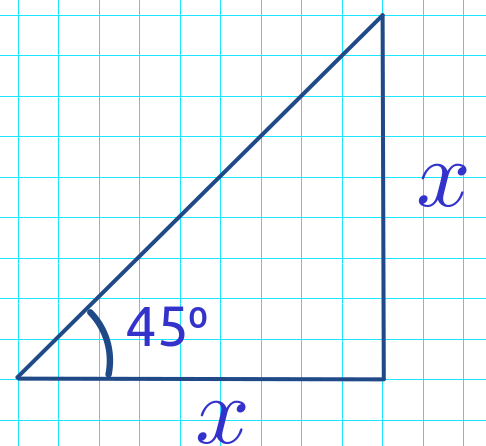
\includegraphics[width=4.5cm]{tals/trig1/img/tan02.png} & $45\degre$ &  \TRAINER{$1 : 1$}\noTRAINER{..........} & $\tan(45\degre) =$ \TRAINER{$1$}\noTRAINER{..........}\\\hline
 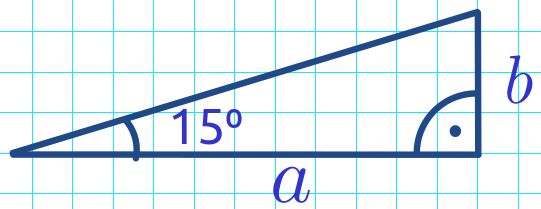
\includegraphics[width=4.5cm]{tals/trig1/img/tan03.png} & $15\degre$ &  \TRAINER{$(2-\sqrt{3}):1$}\noTRAINER{..........} & $\tan(15\degre) \approx$ \TRAINER{$0.2679$}\noTRAINER{..........}\\\hline
\end{tabular}



\newpage

\subsubsection{Arcustangens}
\begin{definition}{Arcustanges}{}
Kennt man das Verhältnis $b:a$ von Gegenkathete $b$ zur Ankathete $a$,
so kann der Winkel $\beta$ mit der \textbf{Umkehrung des Tanges}, des
sog.
\begin{center}Arcustangens\end{center}
  ermittelt werden.
  
\end{definition}


\newpage

\olatLinkArbeitsblatt{Tangens}{https://olat.bbw.ch/auth/RepositoryEntry/572162090/CourseNode/102901169721727}{3-5 Höhenmessungen}

\olatLinkArbeitsblatt{Sinus/Cosinus/Tangens}{https://olat.bbw.ch/auth/RepositoryEntry/572162090/CourseNode/101586242856840}{Täglich
5-10 Minuten}

\youtubeLink{https://www.youtube.com/watch?v=RjFwqJRTgKo}{Mathe Mann
  und das rechtwinklige Dreieck}
\newpage


\subsection{Steigung vs. Winkel}\index{Steigung}
\TadBMTG{95}{Steigungswinkel}
\bbwCenterGraphic{4.5cm}{tals/trig1/img/starkeSteigung.jpg}

Steigungen werden üblicherweise in \% angegeben. Das obige
Verkehrsschild «starke Steigung» gibt 10\% an. Das heißt:

\TNT{3.6}{Auf einen horizontalen Meter, steigt die Straße um 10cm (=
  10\%).
\vspace{3cm}}

Um den Winkel zu berechnen, kann der Tangens verwendet werden:
$$\frac{0.10m}{1.00m} = \tan(\sigma)$$
In obigem Beispiel ist der Steigungswinkel also durch den $\arctan()$
berechenbar:

$$\sigma = \arctan\left(\frac{0.1m}{1.0m}\right) = \arctan(0.1) \approx 5.71\degre$$

\subsection*{Aufgaben}
\AadBMTG{100}{16. a) c), 17. a) c), 18. a) c) und 20.}
\newpage


%% Sinushand

\subsection{Merkregel der wichtigsten Sinus-Werte}\index{Sinushand}

Anstelle des Ablesens im Gleichseitigen Dreieck kann man sich die wichtigsten Werte
auch mit folgender «Sinushand» merken:

\TRAINER{\bbwCenterGraphic{12cm}{tals/trig1/img/sinushand.png}}%% END TRAINER
\noTRAINER{\vspace{98mm}}%%


\TRAINER{%%
\begin{tabular}{r|l|c|l}
      & $sin()$                              & $\cos()$             & $\tan()=\frac{\sin()}{\cos()}$              \\\hline
   0  & $\frac{\sqrt{\textbf{0}}}{2} = 0$    & 1                    &   0                                         \\\hline
  30  & $\frac{\sqrt{\textbf{1}}}{2} = 0.5 $ & $\frac{\sqrt{3}}{2}$ &  $\frac{1}{\sqrt{3}} = \frac{\sqrt{3}}{3}$  \\\hline
  45  & $\frac{\sqrt{\textbf{2}}}{2}$        & $\frac{\sqrt{2}}{2}$ &   1                                         \\\hline
  60  & $\frac{\sqrt{\textbf{3}}}{2}$        & 0.5                  &  $\sqrt{3}$                                 \\\hline
  90  & $\frac{\sqrt{\textbf{4}}}{2} = 1$    & 0                    & nicht definiert
\end{tabular}
}%% END TRAINER

\noTRAINER{%%
\begin{tabular}{r|l|c|l}
      & $sin()$  & $\cos()$  &  $\tan()=\frac{\sin()}{\cos()}$        \\\hline
   0  &          &           &         \\\hline
  30  &          &           &         \\\hline
  45  &          &           &         \\\hline
  60  &          &           &         \\\hline
  90  &          &           &         \\
\end{tabular}
}%% END noTRANIER
\newpage

\subsection*{Aufgaben}
\AadBMTG{100ff}{21., 23., 27., 30. b), 32., 33., 36. und 40. (Winkel bei
  Aufgabe 40. sind im Bogenmaß gegeben.)}
%%\TALSAadBFWG{84ff}{2. alle 3. a) b) e) 4. a) c) 6. a) 8. 9. 15. 23. 26. a) b) c) 30.}%

\newpage
